\documentclass[a4paper,14pt, unknownkeysallowed]{extreport}

\usepackage{cmap} % Улучшенный поиск русских слов в полученном pdf-файле
\usepackage[T2A]{fontenc} % Поддержка русских букв
\usepackage[utf8]{inputenc} % Кодировка utf8
\usepackage[english,russian]{babel} % Языки: русский, английский
\usepackage{enumitem}


\usepackage{threeparttable}

\usepackage[14pt]{extsizes}

\usepackage{caption}
\captionsetup{labelsep=endash}
\captionsetup[figure]{name={Рисунок}}

% \usepackage{ctable}
% \captionsetup[table]{justification=raggedleft,singlelinecheck=off}

\usepackage{amsmath}

\usepackage{geometry}
\geometry{left=30mm}
\geometry{right=15mm}
\geometry{top=20mm}
\geometry{bottom=20mm}

\usepackage{titlesec}
\titleformat{\section}
	{\normalsize\bfseries}
	{\thesection}
	{1em}{}
\titlespacing*{\chapter}{0pt}{-30pt}{8pt}
\titlespacing*{\section}{\parindent}{*4}{*4}
\titlespacing*{\subsection}{\parindent}{*4}{*4}

\usepackage{setspace}
\onehalfspacing % Полуторный интервал

\frenchspacing
\usepackage{indentfirst} % Красная строка
\setlength{\parindent}{1.25cm}

\usepackage{titlesec}
\titleformat{\chapter}{\LARGE\bfseries}{\thechapter}{20pt}{\LARGE\bfseries}
\titleformat{\section}{\Large\bfseries}{\thesection}{20pt}{\Large\bfseries}

\usepackage{multirow}
\usepackage{listings}
\usepackage{xcolor}

% Для листинга кода:
\lstset{ %
language=caml,                 % выбор языка для подсветки (здесь это С)
basicstyle=\small\sffamily, % размер и начертание шрифта для подсветки кода
numbers=left,               % где поставить нумерацию строк (слева\справа)
stepnumber=1,                   % размер шага между двумя номерами строк
numbersep=5pt,                % как далеко отстоят номера строк от подсвечиваемого кода
showspaces=false,            % показывать или нет пробелы специальными отступами
showstringspaces=false,      % показывать или нет пробелы в строках
showtabs=false,             % показывать или нет табуляцию в строках
frame=single,              % рисовать рамку вокруг кода
tabsize=2,                 % размер табуляции по умолчанию равен 2 пробелам
captionpos=t,              % позиция заголовка вверху [t] или внизу [b] 
breaklines=true,           % автоматически переносить строки (да\нет)
breakatwhitespace=false, % переносить строки только если есть пробел
escapeinside={\#*}{*)}   % если нужно добавить комментарии в коде
}



% plot
\usepackage{graphicx}
\usepackage{pgfplots}
\usepackage{filecontents}
\usetikzlibrary{datavisualization}
\usetikzlibrary{datavisualization.formats.functions}

\graphicspath{ {img/} }


\usepackage{subcaption}

\captionsetup{labelsep=endash}
\captionsetup[figure]{name={Рисунок}}



\usepackage[justification=centering]{caption} % Настройка подписей float объектов

\usepackage[unicode,pdftex]{hyperref} % Ссылки в pdf
\hypersetup{hidelinks}

\usepackage{csvsimple}

\newcommand{\code}[1]{\texttt{#1}}

\begin{document}
	
\begin{titlepage}
	\newgeometry{pdftex, left=2cm, right=2cm, top=2.5cm, bottom=2.5cm}
	\fontsize{12pt}{12pt}\selectfont
	\noindent \begin{minipage}{0.15\textwidth}
		
\includegraphics[width=\linewidth]{img/main_logo.jpg}
	\end{minipage}
	\noindent\begin{minipage}{0.9\textwidth}\centering
		\textbf{Министерство науки и высшего образования Российской Федерации}\\
		\textbf{Федеральное государственное бюджетное образовательное учреждение высшего образования}\\
		\textbf{«Московский государственный технический университет имени \newline Н. Э. Баумана}\\
		\textbf{(национальный исследовательский университет)»}\\
		\textbf{(МГТУ им. Н. Э.~Баумана)}
	\end{minipage}
	
	\noindent\rule{18cm}{3pt}
	\newline\newline
	\noindent ФАКУЛЬТЕТ $\underline{\text{«Информатика и системы управления»~~~~~~~~~~~~~~~~~~~~~~~~~~~~~~~~~~~~~~~~~~~~~~~~~~~~~~~}}$ \newline\newline
	\noindent КАФЕДРА $\underline{\text{«Программное обеспечение ЭВМ и информационные технологии»~~~~~~~~~~~~~~~~~~~~~~~}}$\newline\newline\newline\newline\newline\newline\newline
	
	
	\begin{center}
		\noindent\begin{minipage}{1.3\textwidth}\centering
		\Large\textbf{   ~~~ Домашнее задание №1}\newline
		\textbf{по дисциплине "Анализ Алгоритмов"}\newline\newline\newline
		\end{minipage}
	\end{center}
	
	\noindent\textbf{Тема} 			$\underline{\text{Графовые представление}}$\newline\newline
	\noindent\textbf{Студент} 		$\underline{\text{Светличная А.А.}}$\newline\newline
	\noindent\textbf{Группа} 		$\underline{\text{ИУ7-53Б}}$\newline\newline
	\noindent\textbf{Преподаватель} $\underline{\text{Волкова Л. Л., Строганов Ю.В.}}$\newline
	
	\begin{center}
		\vfill
		Москва~---~\the\year
		~г.
	\end{center}
	\restoregeometry
\end{titlepage}
	
	\setcounter{page}{2}
	\tableofcontents
	
\newpage
	
\chapter{Практическая часть}

В данном разделе будут представлен код алгоритма Дейкстры, а также его графовые представления.

\section{Средства реализации}
В домашней работе для реализации алгоритма был выбран язык программирования Python в силу простоты синтаксиса, что позволяет реализовать некоторые ыункции и операции легче, чем, например, на языке программирования C, на котором были реализованы предыдущие лабораторные работы. 

\clearpage

\section{Реализация алгоритма}

В листинге \ref{dijkstra} приведена реализации алгоритма Дейкстры.

\begin{lstlisting}[label= time,caption=Функции замеров процессорного времени,language=python]
    def dijkstra(graph, start):
        rows = len(graph)                                      #1
        columns = len(graph[0])                                #2

        dists = [inf] * rows                                   #3
        dists[start] = 0                                       #4 

        queue = [i for i in range(rows)]                       #5

        while queue:                                           #6
            minVal = inf                                       #7
            minInd = -1                                        #8

            for i, dist in enumerate(dists):                   #9
                if dist < minVal and i in queue:               #10
                    minVal = dist                              #11
                    minInd = i                                 #12

        queue.remove(minInd)                                   #13

        for i in range(columns):                               #14
            if graph[minInd][i] and i in queue:                #15
                newDist = dists[minInd] + graph[minInd][i]     #16
                if newDist < dists[i]:                         #17
                    dists[i] = newDist                         #18

    return dists

\end{lstlisting}
 
\section{Графовые представления}
		
На рисунках \ref{fig:op}, \ref{fig:info}, \ref{fig:op_hist}, \ref{fig:info_hist1} -- \ref{fig:info_hist3} представлены операционный и информационный графы, а также графы операционной и информационной историй соответсвенно для реализации алгоритма Дейкстры.

\begin{figure}[h!]
	\centering
	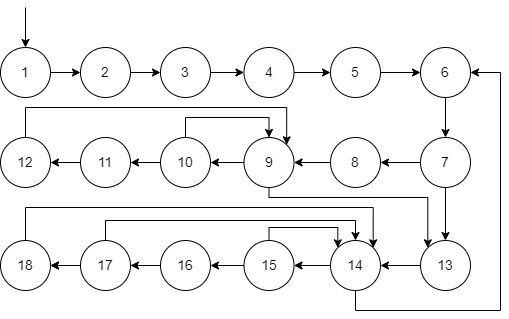
\includegraphics[width=1\linewidth]{img/op.png}
	\caption{Операционный граф}
	\label{fig:op}
\end{figure}

\begin{figure}[h!]
	\centering
	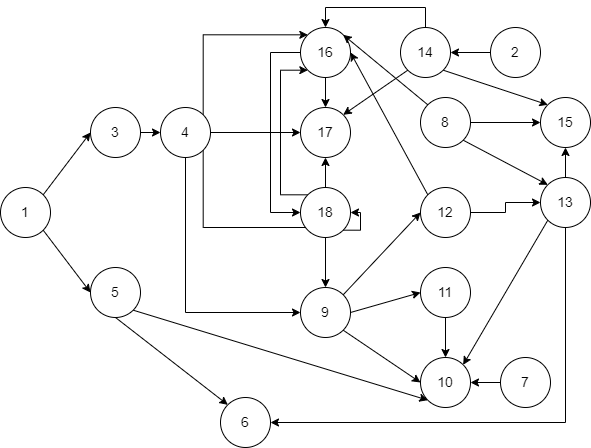
\includegraphics[width=1\linewidth]{img/info.png}
	\caption{Информационный граф}
	\label{fig:info}
\end{figure}

\begin{figure}[h!]
	\centering
	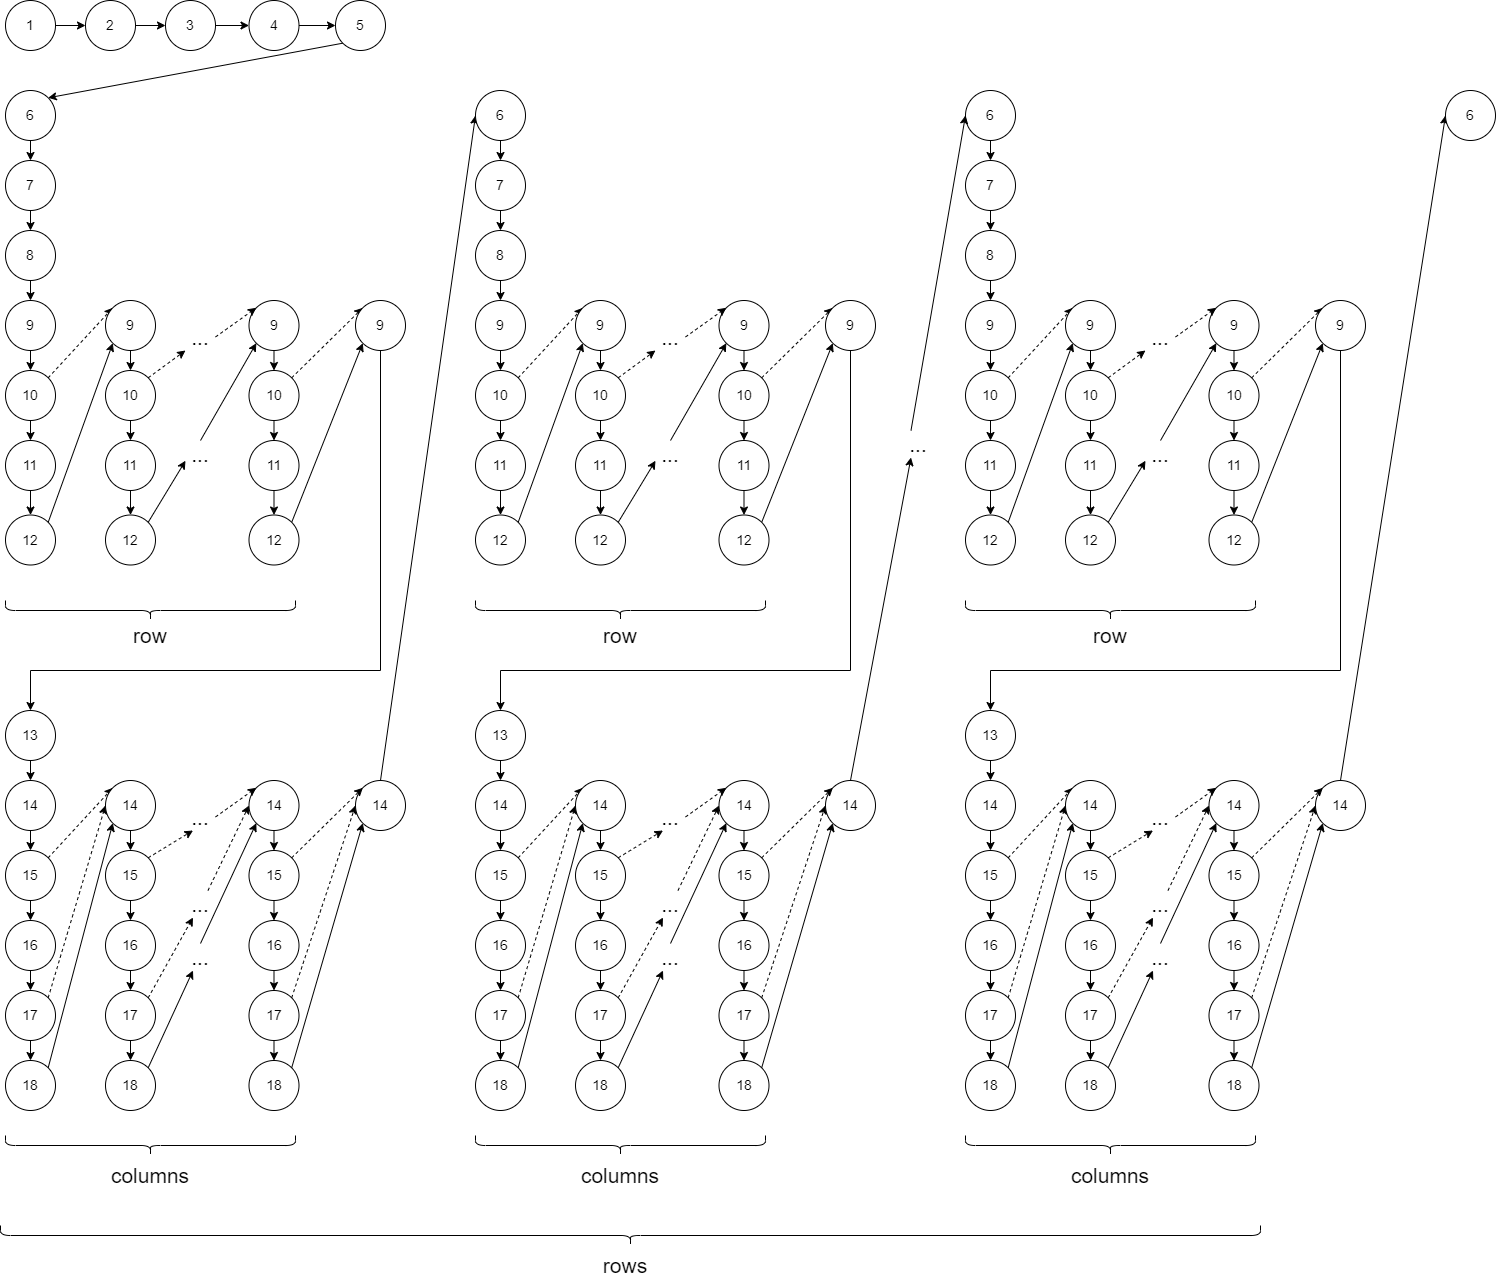
\includegraphics[width=1\linewidth]{img/op_hist.png}
	\caption{Граф операционной истории}
	\label{fig:op_hist}
\end{figure}

\begin{figure}[h!]
	\centering
	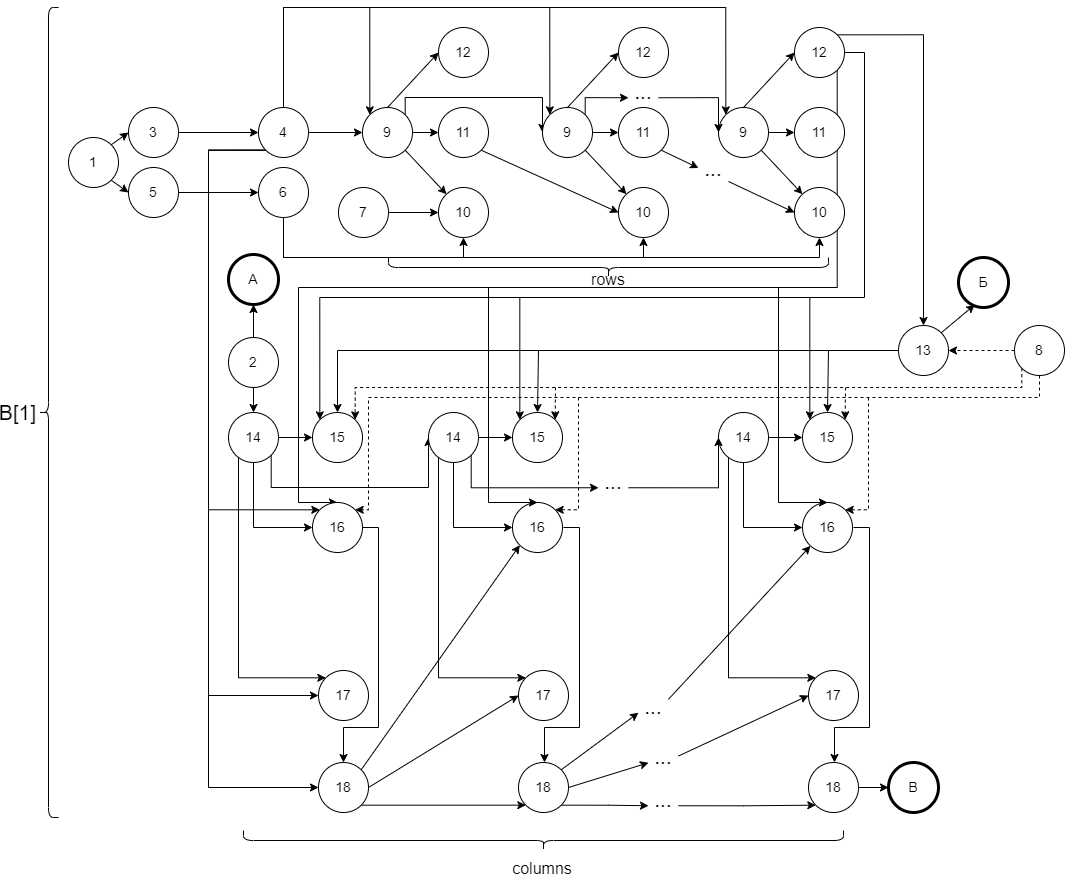
\includegraphics[width=1\linewidth]{img/info_hist1.png}
	\caption{Граф информационной истории (часть 1)}
	\label{fig:info_hist1}
\end{figure}

\begin{figure}[h!]
	\centering
	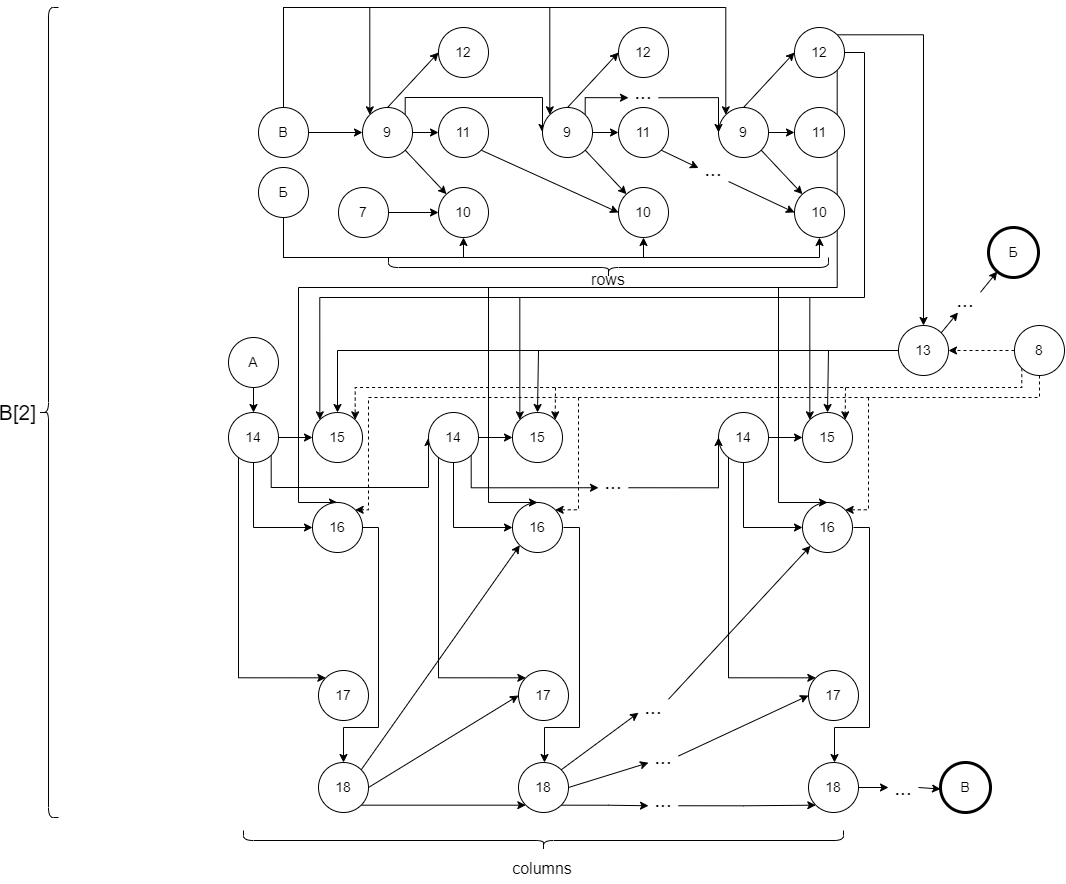
\includegraphics[width=1\linewidth]{img/info_hist2.png}
	\caption{Граф информационной истории (часть 2)}
	\label{fig:info_hist2}
\end{figure}

\begin{figure}[h!]
	\centering
	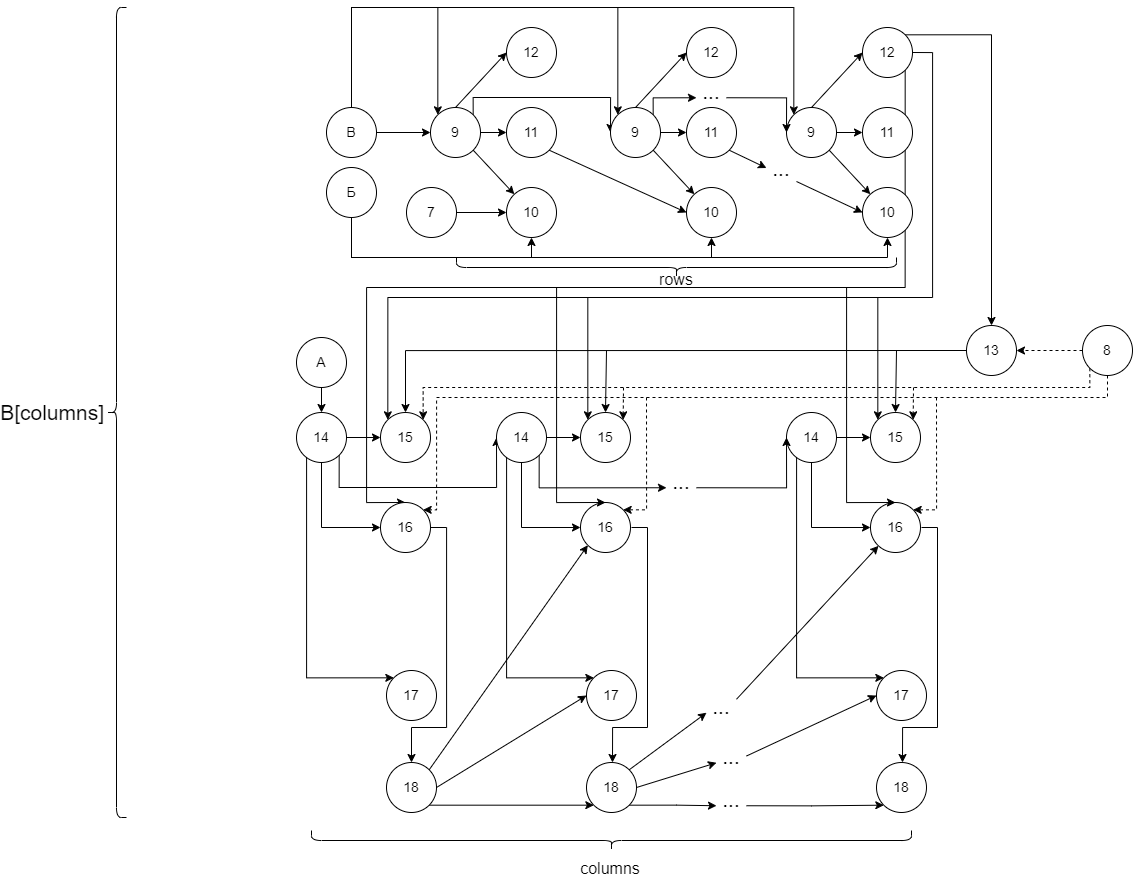
\includegraphics[width=1\linewidth]{img/info_hist3.png}
	\caption{Граф информационной истории (часть 3)}
	\label{fig:info_hist3}
\end{figure}

\chapter{Вывод}
В данной работы были построены графовые представления для алгоритма Дейкстры.
 
\end{document}
